\documentclass{beamer}
\usepackage[utf8]{inputenc}
\usepackage{graphicx, epsfig}
\usepackage{amsmath,mathrsfs,amsfonts,amssymb}
\usepackage{floatflt}
\usepackage{epic,ecltree}
\usepackage{mathtext}
\usepackage{fancybox}
\usepackage{fancyhdr}
\usepackage{multirow}
\usepackage{enumerate}
\usepackage{epstopdf}
\usepackage{multicol}
\usepackage{algorithm}
\usepackage[noend]{algorithmic}
\usepackage{tikz}
\usepackage{blindtext}
\usetheme{default}%{Singapore}%{Warsaw}%{Warsaw}%{Darmstadt}
\usecolortheme{default}

\setbeamerfont{title}{size=\Huge}
\setbeamertemplate{footline}[page number]{}

\setbeamertemplate{section in toc}[sections numbered]


\makeatletter
\newcommand\HUGE{\@setfontsize\Huge{35}{40}}
\makeatother    

\setbeamerfont{title}{size=\HUGE}
\beamertemplatenavigationsymbolsempty

% latin bold lower
\newcommand{\ba}{\mathbf{a}} 
\newcommand{\bc}{\mathbf{c}} 
\newcommand{\be}{\mathbf{e}} 
\newcommand{\bff}{\mathbf{f}} % \bf - for bold type
\newcommand{\bg}{\mathbf{g}} 
\newcommand{\bh}{\mathbf{h}} 
\newcommand{\bp}{\mathbf{p}} 
\newcommand{\bq}{\mathbf{q}} 
\newcommand{\bt}{\mathbf{t}} 
\newcommand{\bs}{\mathbf{s}} 
\newcommand{\bu}{\mathbf{u}} 
\newcommand{\bv}{\mathbf{v}} 
\newcommand{\bw}{\mathbf{w}} 
\newcommand{\bx}{\mathbf{x}} 
\newcommand{\by}{\mathbf{y}} 
\newcommand{\bz}{\mathbf{z}} 

% latin bold upper
\newcommand{\bA}{\mathbf{A}} 
\newcommand{\bB}{\mathbf{B}} 
\newcommand{\bC}{\mathbf{C}} 
\newcommand{\bG}{\mathbf{G}} 
\newcommand{\bI}{\mathbf{I}} 
\newcommand{\bJ}{\mathbf{J}} 
\newcommand{\bL}{\mathbf{L}} 
\newcommand{\bM}{\mathbf{M}} 
\newcommand{\bP}{\mathbf{P}}
\newcommand{\bQ}{\mathbf{Q}} 
\newcommand{\bR}{\mathbf{R}} 
\newcommand{\bT}{\mathbf{T}} 
\newcommand{\bU}{\mathbf{U}} 
\newcommand{\bV}{\mathbf{V}} 
\newcommand{\bW}{\mathbf{W}} 
\newcommand{\bX}{\mathbf{X}} 
\newcommand{\bY}{\mathbf{Y}} 
\newcommand{\bZ}{\mathbf{Z}} 

% latin cal upper
\newcommand{\cF}{\mathcal{F}} 
\newcommand{\cG}{\mathcal{G}} 
\newcommand{\cI}{\mathcal{I}} 
\newcommand{\cL}{\mathcal{L}} 
\newcommand{\cM}{\mathcal{M}} 
\newcommand{\cN}{\mathcal{N}} 
\newcommand{\cP}{\mathcal{P}} 
\newcommand{\cS}{\mathcal{S}} 
\newcommand{\cT}{\mathcal{T}} 
\newcommand{\cW}{\mathcal{W}} 
\newcommand{\cX}{\mathcal{X}} 
\newcommand{\cZ}{\mathcal{Z}} 

% latin bb upper
\newcommand{\bbE}{\mathbb{E}} 
\newcommand{\bbI}{\mathbb{I}} 
\newcommand{\bbP}{\mathbb{P}} 
\newcommand{\bbR}{\mathbb{R}} 

% greek bold lower
\newcommand{\bepsilon}{\boldsymbol{\epsilon}} 
\newcommand{\btheta}{\boldsymbol{\theta}} 
\newcommand{\blambda}{\boldsymbol{\lambda}} 
\newcommand{\bpi}{\boldsymbol{\pi}} 
\newcommand{\bmu}{\boldsymbol{\mu}} 
\newcommand{\bsigma}{\boldsymbol{\sigma}} 
\newcommand{\bphi}{\boldsymbol{\phi}} 

% greek bold upper
\newcommand{\bSigma}{\boldsymbol{\Sigma}} 

\DeclareMathOperator*{\argmin}{arg\,min}
\DeclareMathOperator*{\argmax}{arg\,max}

\newcommand{\createdgmtitle}[1]{\title[\hbox to 56mm{Deep Generative Models  \hfill\insertframenumber\,/\,\inserttotalframenumber}]
	{\vspace{1cm} \\ \textbf{Deep Generative Models} \\ {\Huge Lecture #1}}
	\author{Roman Isachenko}
		\institute{
\includegraphics[width=0.7cm]{../utils/aimasterslogo} \LARGE{AI Masters}}
	\date{2024, Spring}
}

\usepackage{tikz}
\usetikzlibrary{arrows,shapes,positioning,shadows,trees}

\newcommand\myfootnote[1]{%
  \tikz[remember picture,overlay]
  \draw (current page.south west) +(1in + \oddsidemargin,0.5em)
  node[anchor=south west,inner sep=0pt]{\parbox{\textwidth}{%
      \rlap{\rule{10em}{0.4pt}}\raggedright\scriptsize \textit{#1}}};}

\newcommand\myfootnotewithlink[2]{%
  \tikz[remember picture,overlay]
  \draw (current page.south west) +(1in + \oddsidemargin,0.5em)
  node[anchor=south west,inner sep=0pt]{\parbox{\textwidth}{%
      \rlap{\rule{10em}{0.4pt}}\raggedright\scriptsize\href{#1}{\textit{#2}}}};}
      
\AtBeginSection[]
      {
      	\begin{frame}{Outline}
      		\tableofcontents[currentsection]
      	\end{frame}
      }
      \AtBeginSubsection[]{
      	\begin{frame}{Outline}
      		\tableofcontents[currentsection,currentsubsection]
      	\end{frame}
}
\createdgmtitle{12}

\usepackage{tikz}

\usetikzlibrary{arrows,shapes,positioning,shadows,trees}
%--------------------------------------------------------------------------------
\begin{document}
%--------------------------------------------------------------------------------
\begin{frame}[noframenumbering,plain]
%\thispagestyle{empty}
\titlepage
\end{frame}
%=======
\begin{frame}{Recap of previous lecture}
	\begin{block}{Continuous-in-time dynamic (neural ODE)}
		\vspace{-0.7cm}
		\begin{align*}
		   \frac{d \bz(t)}{dt} &= \bff_{\btheta}(\bz(t), t); \quad \text{with initial condition }\bz(0) = \bz_0. \\
		   \bz(t_1) &= \int^{1}_{0} \bff_{\btheta}(\bz(t), t) d t  + \bz_0 \approx \text{ODESolve}(\bz(0), \bff_{\btheta}, t_0=0, t_1=1).
		\end{align*}
		\vspace{-0.7cm}
	\end{block}	
	\begin{block}{Euler update step}
		\vspace{-0.6cm}
		\[
   \frac{\bz(t + \Delta t) - \bz(t)}{\Delta t} = \bff_{\btheta}(\bz(t), t) \,\, \Rightarrow \,\, \bz(t + \Delta t) = \bz(t) + \Delta t \cdot \bff_{\btheta}(\bz(t), t)
		\]
		\vspace{-0.7cm}
	\end{block}	
	\begin{block}{Theorem (Picard)}
		If $\bff$ is uniformly Lipschitz continuous in $\bz$ and continuous in $t$, then the ODE has a \textbf{unique} solution.
	\end{block}
		\vspace{-0.7cm}
		\begin{align*}
			\bx &= \bz(1) = \bz(0) + \int_{0}^{1} \bff_{\btheta}(\bz(t), t) dt \\
			\bz &= \bz(0) = \bz(1) + \int_{1}^{0} \bff_{\btheta}(\bz(t), t) dt
		\end{align*}
	\myfootnotewithlink{https://arxiv.org/abs/1806.07366}{Chen R. T. Q. et al. Neural Ordinary Differential Equations, 2018}   
\end{frame}
%=======
\begin{frame}{Recap of previous lecture}
	\begin{block}{Theorem (Kolmogorov-Fokker-Planck: special case)}
		If $\bff$ is uniformly Lipschitz continuous in $\bz$ and continuous in $t$, then
		\[
			\frac{d \log p(\bz(t), t)}{d t} = - \text{tr} \left( \frac{\partial \bff_{\btheta}(\bz(t), t)}{\partial \bz(t)} \right).
		\]
		\[
			\log p_1(\bz(1)) = \log p_0(\bz(0)) - \int_{0}^{1} \text{tr}  \left( \frac{\partial \bff_{\btheta}(\bz(t), t)}{\partial \bz(t)} \right) dt.
		\]
	\end{block}
	\vspace{-0.3cm}
	\begin{itemize}
		\item \textbf{Discrete-in-time NF}: evaluation of determinant of the Jacobian costs $O(m^3)$ (we need invertible $\bff$).
		\item \textbf{Continuous-in-time NF}: getting the trace of the Jacobian costs $O(m^2)$ (we need smooth $\bff$).
	\end{itemize}
	\begin{block}{Hutchinson's trace estimator}
		\vspace{-0.3cm}
		\[
  \log p_1(\bz(1)) = \log p_0(\bz(0)) - \mathbb{E}_{p(\bepsilon)} \int_{0}^{1} \left[ {\color{violet}\bepsilon^T \frac{\partial \bff}{\partial \bz}} \bepsilon \right] dt.
		\]
	\end{block}
	\myfootnotewithlink{https://arxiv.org/abs/1810.01367}{Grathwohl W. et al. FFJORD: Free-form Continuous Dynamics for Scalable Reversible Generative Models, 2018} 
\end{frame}
%=======
\begin{frame}{Recap of previous lecture}
	\begin{block}{Forward pass (Loss function)}
		\vspace{-0.3cm}
		\[
			\bz = \bx + \int_{1}^{0} \bff_{\btheta}(\bz(t), t) dt, \quad L(\bz) = - \log p(\bx | \btheta)
		\]
		\[
			L(\bz) = - \log p(\bz) + \int_{0}^{1} \text{tr} \left( \frac{\partial \bff_{\btheta}(\bz(t), t)}{\partial \bz(t)} \right) dt
		\]
		\vspace{-0.5cm}
	\end{block}
	\begin{block}{Adjoint functions}
		\vspace{-0.4cm}
		\[
			\ba_{\bz}(t) = \frac{\partial L}{\partial \bz(t)}; \quad \ba_{\btheta}(t) = \frac{\partial L}{\partial \btheta(t)}.
		\]
		These functions show how the gradient of the loss depends on the hidden state~$\bz(t)$ and parameters $\btheta$.
		\vspace{-0.3cm}
	\end{block}

	\begin{block}{Theorem (Pontryagin)}
		\vspace{-0.6cm}
		\[
		\frac{d \ba_{\bz}(t)}{dt} = - \ba_{\bz}(t)^T \cdot \frac{\partial \bff_{\btheta}(\bz(t), t)}{\partial \bz}; \quad \frac{d \ba_{\btheta}(t)}{dt} = - \ba_{\bz}(t)^T \cdot \frac{\partial \bff_{\btheta}(\bz(t),  t)}{\partial \btheta}.
		\]
		\vspace{-0.7cm}
	\end{block}

	\myfootnotewithlink{https://arxiv.org/abs/1806.07366}{Chen R. T. Q. et al. Neural Ordinary Differential Equations, 2018}     
\end{frame}
%=======
\begin{frame}{Recap of previous lecture}
	\begin{block}{Forward pass}
		\vspace{-0.3cm}
		\[
		\bz = \bz(0) = \int^{1}_{0} \bff_{\btheta}(\bz(t), t) d t  + \bx \quad \Rightarrow \quad \text{ODE Solver}
		\]
		\vspace{-0.4cm}
	\end{block}
	\begin{block}{Backward pass}
		\vspace{-0.5cm}
		\begin{equation*}
			\left.
			{\footnotesize 
				\begin{aligned}
					\frac{\partial L}{\partial \btheta(t_1)} &= \ba_{\btheta}(1) =  - \int_{0}^{1} \ba_{\bz}(t)^T \frac{\partial \bff_{\btheta}(\bz(t), t)}{\partial \btheta(t)} dt + 0 \\
					\frac{\partial L}{\partial \bz(1)} &= \ba_{\bz}(1) =  - \int_{0}^{1} \ba_{\bz}(t)^T \frac{\partial \bff_{\btheta}(\bz(t), t)}{\partial \bz(t)} dt + \frac{\partial L}{\partial \bz(0)} \\
					\bz(1) &= - \int^{0}_{1} \bff_{\btheta}(\bz(t), t) d t  + \bz_0.
				\end{aligned}
			}
			\right\rbrace
			\Rightarrow
			\text{ODE Solver}
		\end{equation*}
		\vspace{-0.4cm} 
	\end{block}
	\textbf{Note:} These scary formulas are the standard backprop in the discrete case.
	\myfootnotewithlink{https://arxiv.org/abs/1806.07366}{Chen R. T. Q. et al. Neural Ordinary Differential Equations, 2018}   
\end{frame}
%=======
\begin{frame}{Recap of previous lecture}
	\vspace{-0.2cm}
	\begin{block}{SDE basics}
		Let define stochastic process $\bx(t)$ with initial condition $\bx(0) \sim p_0(\bx)$:
		\[
			d\bx = \mathbf{f}(\bx, t) dt + g(t) d \bw, 
		\]
		where $\bw(t)$ is the standard Wiener process (Brownian motion)
		\vspace{-0.2cm}
		\[		
			\bw(t) - \bw(s) \sim \cN(0, (t - s) \bI), \quad d \bw = \bepsilon \cdot \sqrt{dt}, \, \text{where } \bepsilon \sim \cN(0, \bI).
		\]
	\end{block}
	\vspace{-0.3cm}
	\begin{block}{Discretization of SDE (Euler method)}
		\vspace{-0.3cm}
		\[
			\bx(t + dt) = \bx(t) + \bff(\bx(t), t) \cdot dt + g(t) \cdot \bepsilon \cdot \sqrt{dt}
		\]
		\vspace{-0.3cm}
	\end{block}
	\begin{itemize}
		\item At each moment $t$ we have the density $p_t(\bx) = p(\bx, t)$.
		\item $p: \bbR^m \times [0, 1] \rightarrow \bbR_+$ is a \textbf{probability path} between $p_0(\bx)$ and $p_1(\bx)$.
	\end{itemize}
\end{frame}
%=======
\begin{frame}{Recap of previous lecture}
 	\begin{block}{Theorem (Kolmogorov-Fokker-Planck)}
 		Evolution of the distribution $p_t(\bx)$ is given by the following equation:
 		\vspace{-0.3cm}
 		\[
 			\frac{\partial p_t(\bx)}{\partial t} = - \text{div}\left(\bff(\bx, t) p_t(\bx)\right) + \frac{1}{2}g^2(t) \Delta_{\bx}p_t(\bx)
 		\]
 		\vspace{-0.5cm}
 	\end{block}
 	\begin{block}{Langevin SDE (special case)}
 		\vspace{-0.3cm}
 		\[
 			d \bx = {\color{violet}\frac{1}{2} \frac{\partial}{\partial \bx} \log p_t(\bx)} d t + {\color{teal} 1 } \cdot d \bw
 		\]
 		\vspace{-0.3cm}
 	\end{block}
 	The density $p(\bx | \btheta)$ is a \textbf{stationary} distribution for the SDE.
	\begin{block}{Langevin dynamics}
		Samples from the following dynamics will comes from $p(\bx | \btheta)$ under mild regularity conditions for small enough $\eta$.
		\vspace{-0.2cm}
		\[
			\bx_{t + 1} = \bx_t + \eta \frac{1}{2} \nabla_{\bx_t} \log p(\bx_t | \btheta) + \sqrt{\eta} \cdot \bepsilon, \quad \bepsilon \sim \cN(0, \bI).
		\]
	\end{block}
	\myfootnotewithlink{https://www.stats.ox.ac.uk/~teh/research/compstats/WelTeh2011a.pdf}{Welling M. Bayesian Learning via Stochastic Gradient Langevin Dynamics, 2011}
\end{frame}
%=======
\begin{frame}{Outline}
	\tableofcontents
\end{frame}
%=======
\section{Probability flow ODE}
%=======
\begin{frame}{Probability flow ODE}
	\begin{block}{Theorem}
		Assume SDE $d\bx = \mathbf{f}(\bx, t) dt + g(t) d \bw$ induces the probability path~$p_t(\bx)$.
		Then there exists ODE with identical probability path $p_t(\bx)$ of the form
		\vspace{-0.3cm}
		\[
			d\bx = \left[\mathbf{f}(\bx, t) -\frac{1}{2} g^2(t) \frac{\partial}{\partial \bx} \log p_t(\bx) \right] dt
		\]
		\vspace{-0.7cm}
	\end{block}
	\begin{block}{Proof}
 		\vspace{-0.7cm}
 		{\small
 		\begin{multline*}
 			\frac{\partial p_t(\bx)}{\partial t} = \text{tr}\left(- \frac{\partial}{\partial \bx} \bigl[ \mathbf{f}(\bx, t) p_t(\bx)\bigr] + \frac{1}{2} g^2(t) \frac{\partial^2 p_t(\bx)}{\partial \bx^2} \right) = \\
 			=  \text{tr}\left(- \frac{\partial}{\partial \bx} \left[ \mathbf{f}(\bx, t) p_t(\bx) - \frac{1}{2} g^2(t) {\color{violet}\frac{\partial p_t(\bx)}{\partial \bx}} \right]  \right) = \\
			 =  \text{tr}\left(- \frac{\partial}{\partial \bx} \left[ \mathbf{f}(\bx, t) p_t(\bx) - \frac{1}{2} g^2(t) {\color{violet}p_t(\bx) \frac{\partial \log p_t(\bx)}{\partial \bx}} \right]  \right)= \\
		  =  \text{tr}\left(- \frac{\partial}{\partial \bx} \left[ \left( {\color{teal}\mathbf{f}(\bx, t) - \frac{1}{2} g^2(t) \frac{\partial \log p_t(\bx)}{\partial \bx}}\right) p_t(\bx) \right]  \right)
 		\end{multline*}
 		}
 	\end{block}
	\myfootnotewithlink{https://arxiv.org/abs/2011.13456}{Song Y., et al. Score-Based Generative Modeling through Stochastic Differential Equations, 2020}
\end{frame}
%=======
\begin{frame}{Probability flow ODE}
	\begin{block}{Theorem}
		Assume SDE $d\bx = \mathbf{f}(\bx, t) dt + g(t) d \bw$ induces the probability path~$p_t(\bx)$.
		Then there exists ODE with identical probabilities distribution $p_t(\bx)$ of the form
		\vspace{-0.3cm}
		\[
			d\bx = \left[\mathbf{f}(\bx, t) -\frac{1}{2} g^2(t) \frac{\partial}{\partial \bx} \log p_t(\bx) \right] dt
		\]
		\vspace{-0.7cm}
	\end{block}
	\begin{block}{Proof (continued)}
 		\vspace{-0.7cm}
 		\begin{multline*}
 			\frac{\partial p_t(\bx)}{\partial t} =  \text{tr}\left(- \frac{\partial}{\partial \bx} \left[ \left( {\color{teal}\mathbf{f}(\bx, t) - \frac{1}{2} g^2(t) \frac{\partial \log p_t(\bx)}{\partial \bx}}\right) p_t(\bx) \right]  \right) =\\
 			  =  \text{tr}\left(- \frac{\partial}{\partial \bx} \left[ {\color{teal}\tilde{\mathbf{f}}(\bx, t)} p_t(\bx) \right]  \right)
 		\end{multline*}
 	\end{block}
 	\vspace{-1.0cm}
 	\[
 		d \bx = \tilde{\bff}(\bx, t) dt + 0 \cdot d \bw = \left[\mathbf{f}(\bx, t) -\frac{1}{2} g^2(t) \frac{\partial}{\partial \bx} \log p_t(\bx) \right] dt
 	\]
	\myfootnotewithlink{https://arxiv.org/abs/2011.13456}{Song Y., et al. Score-Based Generative Modeling through Stochastic Differential Equations, 2020}
\end{frame}
%=======
\begin{frame}{Probability flow ODE}
	\vspace{-0.5cm}
	\begin{align*}
		d\bx &= \mathbf{f}(\bx, t) dt + g(t) d \bw - \text{SDE} \\
		d\bx &= \left[\mathbf{f}(\bx, t) -\frac{1}{2} g^2(t) \frac{\partial}{\partial \bx} \log p_t(\bx) \right] dt  - \text{probability flow ODE}
	\end{align*}
	\vspace{-0.3cm}
	\begin{itemize}
		\item The term $\bs(\bx, t) = \frac{\partial}{\partial \bx} \log p_t(\bx)$ is a score function for continuous time.
		\item ODE has more stable trajectories.
	\end{itemize}
	\begin{figure}
		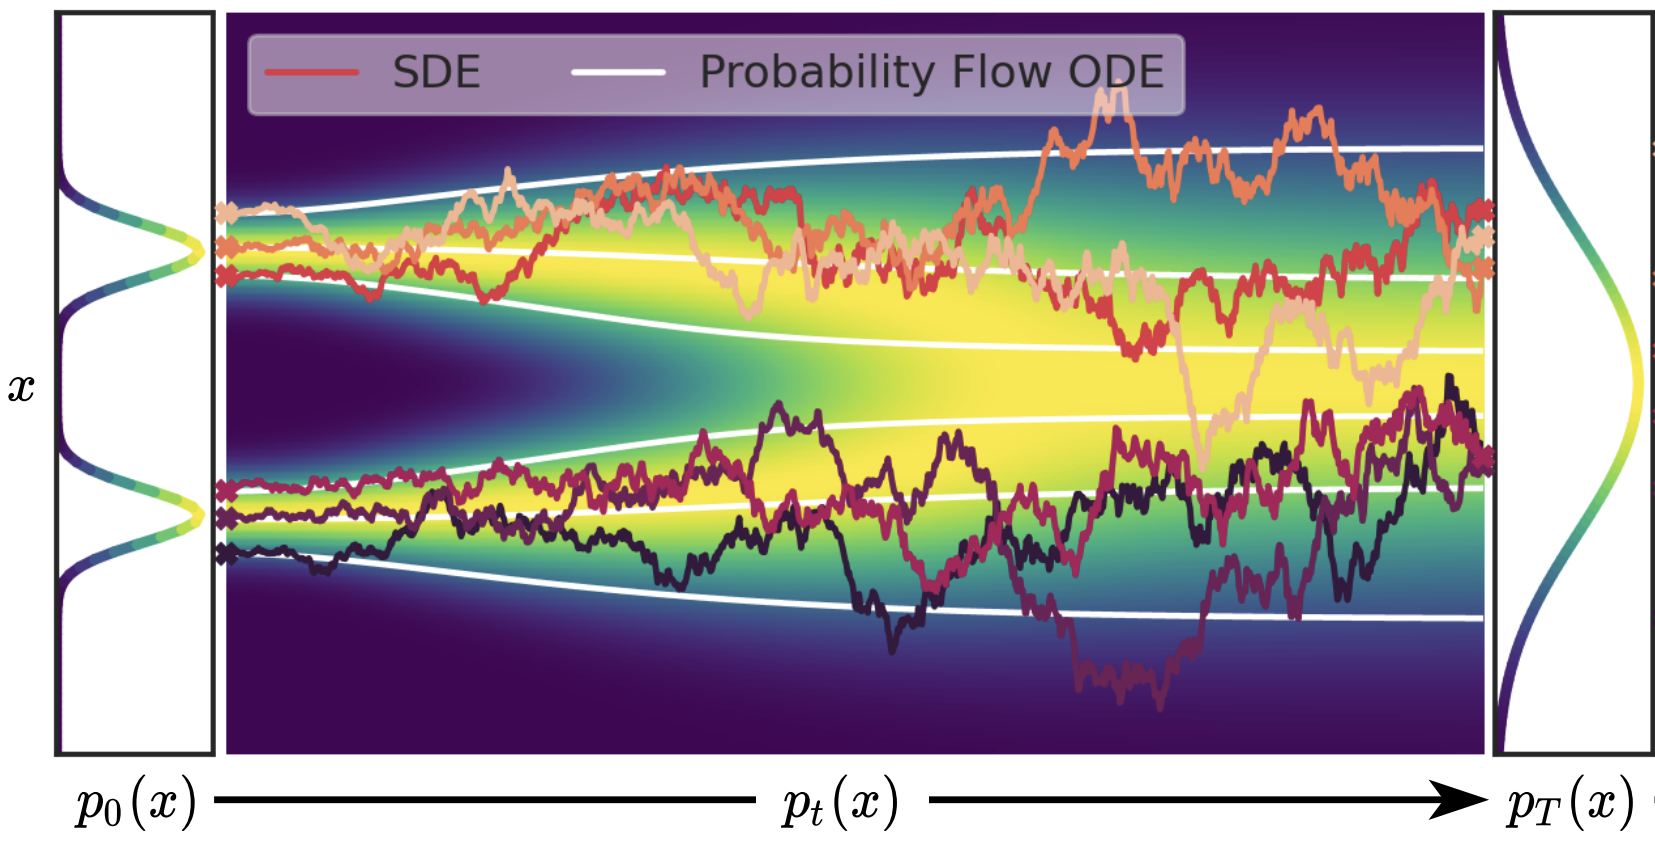
\includegraphics[width=0.75\linewidth]{figs/probability_flow}
	\end{figure}
	\myfootnotewithlink{https://arxiv.org/abs/2011.13456}{Song Y., et al. Score-Based Generative Modeling through Stochastic Differential Equations, 2020}
\end{frame}
%=======
\section{Reverse SDE}
%=======
\begin{frame}{Reverse SDE}
	\vspace{-0.3cm}
	\[
		d\bx = \mathbf{f}(\bx, t) dt, \quad \bx(t + dt) = \bx(t) + \mathbf{f}(\bx, t) dt
	\]
	Here $dt$ could be $>0$ or $<0$. 
	\begin{block}{Reverse ODE}
		Let $\tau = 1 - t$ ($d\tau = -dt$).
		\vspace{-0.3cm}
		\[
			d\bx = - \bff(\bx, 1 - \tau) d \tau
		\]
	\end{block}
	\vspace{-0.5cm}
	\begin{itemize}
		\item How to revert SDE $d\bx = \mathbf{f}(\bx, t) dt + g(t) d \bw$? 
		\item Wiener process gives the randomness that we have to revert.
	\end{itemize}
	\vspace{-0.3cm}
	\begin{block}{Theorem}
		There exists the reverse SDE for the SDE $d\bx = \mathbf{f}(\bx, t) dt + g(t) d \bw$ that has the following form
		\vspace{-0.3cm}
		\[
			d\bx = \left(\mathbf{f}(\bx, t) {\color{violet}- g^2(t) \frac{\partial \log p_t(\bx)}{\partial \bx}}\right) dt + g(t) d \bw
		\]
		\vspace{-0.5cm} \\
		with $dt < 0$.
	\end{block}
	\myfootnotewithlink{https://arxiv.org/abs/2011.13456}{Song Y., et al. Score-Based Generative Modeling through Stochastic Differential Equations, 2020}
\end{frame}
%=======
\begin{frame}{Reverse SDE}
	\begin{block}{Theorem}
		There exists the reverse SDE for the SDE $d\bx = \mathbf{f}(\bx, t) dt + g(t) d \bw$ that has the following form
		\vspace{-0.3cm}
		\[
			d\bx = \left(\mathbf{f}(\bx, t) {\color{violet}- g^2(t) \frac{\partial \log p_t(\bx)}{\partial \bx}}\right) dt + g(t) d \bw
		\]
		\vspace{-0.5cm} \\
		with $dt < 0$.
	\end{block}
	\textbf{Note:} Here we also see the score function $\bs(\bx, t) = \frac{\partial}{\partial \bx} \log p_t(\bx)$.
	\begin{block}{Sketch of the proof}
		\begin{itemize}
			\item Convert initial SDE to probability flow ODE.
			\item Revert probability flow ODE.
			\item Convert reverse probability flow ODE to reverse SDE.
		\end{itemize}
	\end{block}
	\myfootnotewithlink{https://arxiv.org/abs/2011.13456}{Song Y., et al. Score-Based Generative Modeling through Stochastic Differential Equations, 2020}
\end{frame}
%=======
\begin{frame}{Reverse SDE}
	\begin{block}{Proof}
		\begin{itemize}
			\item Convert initial SDE to probability flow ODE
			\vspace{-0.1cm}
			{\footnotesize
			\begin{align*}
				d\bx &= \mathbf{f}(\bx, t) dt + g(t) d \bw \\
				d\bx &= \left[\mathbf{f}(\bx, t) -\frac{1}{2} g^2(t) \frac{\partial}{\partial \bx} \log p_t(\bx) \right] dt
			\end{align*}
			}
			\item Revert probability flow ODE
			\vspace{-0.1cm}
			{\footnotesize
			\begin{align*}
				d\bx &= \left[\mathbf{f}(\bx, t) -\frac{1}{2} g^2(t) \frac{\partial}{\partial \bx} \log p_t(\bx) \right] dt \\
				d\bx &= \left[- \mathbf{f}(\bx, 1 - \tau) + \frac{1}{2} g^2(1 - \tau) \frac{\partial}{\partial \bx} \log p(\bx, 1 - \tau) \right] d \tau
			\end{align*}
			}
			\item Convert reverse probability flow ODE to reverse SDE
			\vspace{-0.1cm}
			{\footnotesize
			\begin{align*}
				d\bx &= \left[- \mathbf{f}(\bx, 1 - \tau) + \frac{1}{2} g^2(1 - \tau) \frac{\partial}{\partial \bx} \log p(\bx, 1 - \tau) \right] d \tau \\
				d\bx &= \left[- \mathbf{f}(\bx, 1 - \tau) + g^2(1 - \tau) \frac{\partial}{\partial \bx} \log p(\bx, 1 - \tau) \right] d\tau + g(1 - \tau) d \bw
			\end{align*}
			}
		\end{itemize}
	\end{block}
	\myfootnotewithlink{https://arxiv.org/abs/2011.13456}{Song Y., et al. Score-Based Generative Modeling through Stochastic Differential Equations, 2020}
\end{frame}
%=======
\begin{frame}{Reverse SDE}
	\begin{block}{Theorem}
		There exists the reverse SDE for the SDE $d\bx = \mathbf{f}(\bx, t) dt + g(t) d \bw$ that has the following form
		\vspace{-0.3cm}
		\[
			d\bx = \left(\mathbf{f}(\bx, t) {\color{violet}- g^2(t) \frac{\partial \log p_t(\bx)}{\partial \bx}}\right) dt + g(t) d \bw
		\]
		\vspace{-0.5cm} \\
		with $dt < 0$.
	\end{block}
	\begin{block}{Proof (continued)}
		\vspace{-0.7cm}
		\[
			d\bx = \left[- \mathbf{f}(\bx, 1 - \tau) + g^2(1 - \tau) \frac{\partial}{\partial \bx} \log p(\bx, 1 - \tau) \right] d \tau + g(1 - \tau) d \bw
		\]
		\[
			d\bx = \left(\mathbf{f}(\bx, t) - g^2(t) \frac{\partial \log p_t(\bx)}{\partial \bx}\right) dt + g(t) d \bw
		\]
		Here $d\tau > 0$ and $dt < 0$.
	\end{block}
	\myfootnotewithlink{https://arxiv.org/abs/2011.13456}{Song Y., et al. Score-Based Generative Modeling through Stochastic Differential Equations, 2020}
\end{frame}
%=======
\begin{frame}{Reverse SDE}
	\vspace{-0.5cm}
	\begin{align*}
		d\bx &= \mathbf{f}(\bx, t) dt + g(t) d \bw - \text{SDE} \\
		d\bx &= \left[\mathbf{f}(\bx, t) -\frac{1}{2} g^2(t) \frac{\partial}{\partial \bx} \log p_t(\bx) \right] dt - \text{probability flow ODE} \\
		d\bx &= \left(\mathbf{f}(\bx, t) - g^2(t) \frac{\partial \log p_t(\bx)}{\partial \bx}\right) dt + g(t) d \bw - \text{reverse SDE}
	\end{align*}
	\vspace{-0.5cm}
	\begin{itemize}
		\item We got the way to transform one distribution to another via SDE with some probability path $p_t(\bx)$.
		\item We are able to revert this process with the score function.
	\end{itemize}
	\vspace{-0.3cm}
	\begin{figure}
		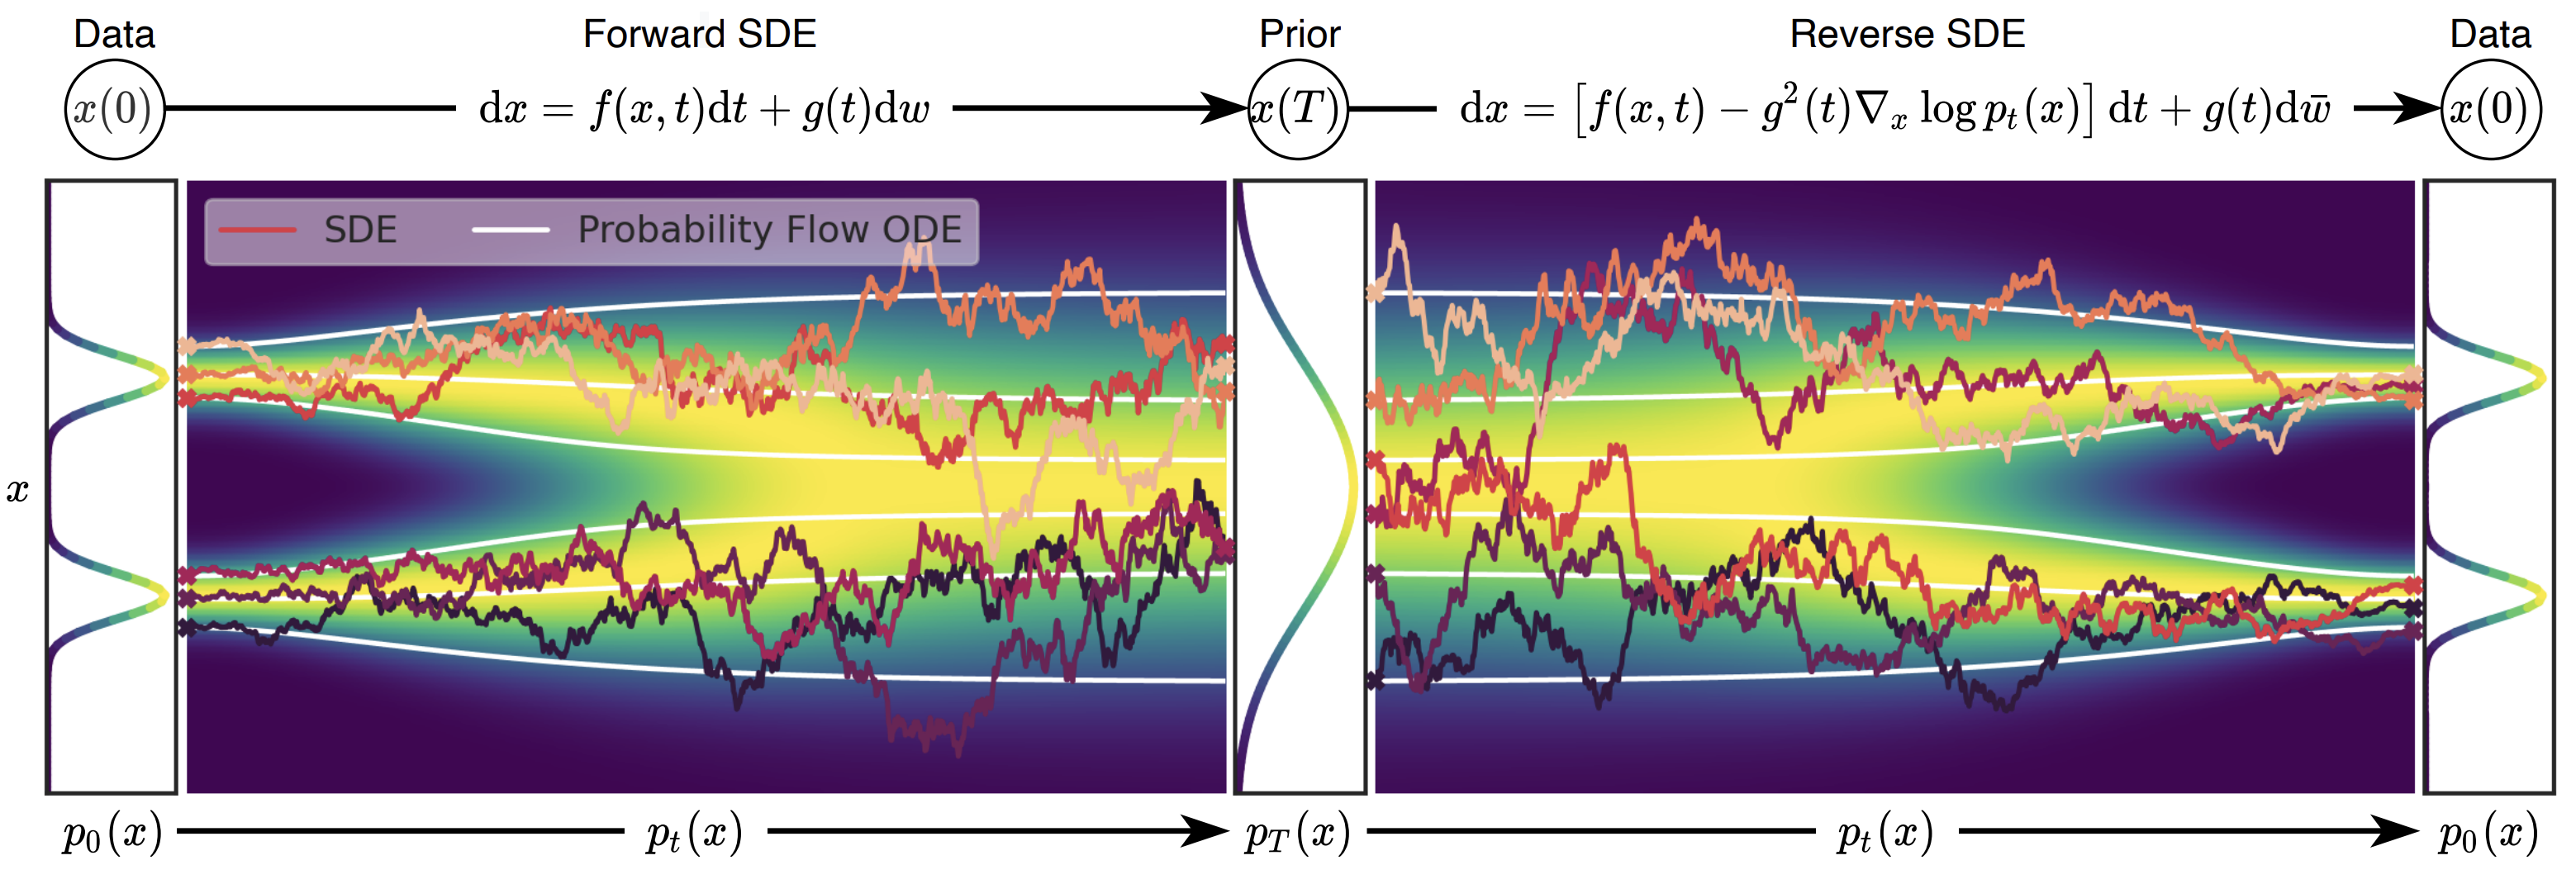
\includegraphics[width=0.9\linewidth]{figs/sde}
	\end{figure}
	\myfootnotewithlink{https://arxiv.org/abs/2011.13456}{Song Y., et al. Score-Based Generative Modeling through Stochastic Differential Equations, 2020}
\end{frame}
%=======
\section{Diffusion and Score matching SDEs}
%=======
\begin{frame}{Score matching SDE}
	\begin{block}{Denoising score matching}
		\vspace{-0.7cm}
		\begin{align*}
			\bx_t &= \bx + \sigma_t \cdot \bepsilon_t, & p(\bx_t | \bx, \sigma_t) &= \cN(\bx, \sigma_t^2 \cdot \bI) \\
			\bx_{t-1} &= \bx + \sigma_{t-1} \cdot \bepsilon_{t-1}, & p(\bx_{t-1} | \bx, \sigma_{t-1}) &= \cN(\bx, \sigma_{t-1}^2 \cdot \bI)
		\end{align*}
	\end{block}
	\vspace{-1.0cm}
	\[
		\bx_t = \bx_{t - 1} + \sqrt{\sigma^2_t - \sigma^2_{t-1}} \cdot \bepsilon, \quad q(\bx_{t} | \bx_{t-1}) = \cN(\bx_{t-1}, (\sigma_t^2 - \sigma_{t-1}^2) \cdot \bI)
	\]
	Let turn this Markov chain to the continuous stochastic process~$\bx(t)$ taking $T \rightarrow \infty$:
	\[
		{\color{teal}\bx(t + dt)} = {\color{teal}\bx(t)} + \sqrt{\frac{\sigma^2(t + dt) - \sigma^2(t)}{dt} {\color{violet}dt}} \cdot {\color{violet}\bepsilon} = \bx(t) + \sqrt{\frac{ d [\sigma^2(t)]}{dt}} \cdot {\color{violet}d \bw}
	\]
	\vspace{-0.5cm}
	\begin{block}{Variance Exploding SDE}
		\vspace{-0.3cm}
		\[
			d \bx = \sqrt{\frac{ d [\sigma^2(t)]}{dt}} \cdot d \bw
		\]
	\end{block}
	\myfootnotewithlink{https://arxiv.org/abs/2011.13456}{Song Y., et al. Score-Based Generative Modeling through Stochastic Differential Equations, 2020}
\end{frame}
%=======
\begin{frame}{Diffusion SDE}
	\begin{block}{Denoising Diffusion}
		\vspace{-0.5cm}
		\[
			\bx_t = \sqrt{1 - \beta_t} \cdot \bx_{t - 1} + \sqrt{\beta_t} \cdot \bepsilon, \quad q(\bx_t | \bx_{t-1}) = \cN(\sqrt{1 - \beta_t} \cdot \bx_{t-1}, \beta_t \cdot \bI)
		\]
		\vspace{-0.5cm}
	\end{block}
	Let turn this Markov chain to the continuous stochastic process taking $T \rightarrow \infty$ and taking $\beta(\frac{t}{T}) = \beta_t \cdot T$
	\begin{multline*}
		{\color{teal}\bx(t)} = \sqrt{1 - \beta(t) dt} \cdot \bx(t - dt) + \sqrt{\beta(t)dt} \cdot \bepsilon \approx \\
		\approx (1 - \frac{1}{2} \beta(t) dt) \cdot \bx(t - dt) + \sqrt{\beta(t){\color{violet}dt}} \cdot {\color{violet}\bepsilon} = \\
		= {\color{teal}\bx(t - dt)} - \frac{1}{2} \beta(t) \bx(t - dt) dt  + \sqrt{\beta(t)} \cdot {\color{violet}d \bw}
	\end{multline*}
	\vspace{-0.5cm}
	\begin{block}{Variance Preserving SDE}
		\vspace{-0.3cm}
		\[
			{\color{teal}d \bx} = - \frac{1}{2} \beta(t) \bx(t) dt + \sqrt{\beta(t)} \cdot d \bw
		\]
	\end{block}
	\myfootnotewithlink{https://arxiv.org/abs/2011.13456}{Song Y., et al. Score-Based Generative Modeling through Stochastic Differential Equations, 2020}
\end{frame}
%=======
\begin{frame}{Diffusion SDE}
	\vspace{-0.3cm}
	\[
		d\bx = \mathbf{f}(\bx, t) dt + g(t) d \bw
	\]
	\vspace{-0.3cm}
	\begin{block}{Variance Exploding SDE (NCSN)}
		\vspace{-0.5cm}
		\[
			d \bx = \sqrt{\frac{ d [\sigma^2(t)]}{dt}} \cdot d \bw, \quad \bff(\bx, t) = 0, \quad g(t) = \sqrt{\frac{ d [\sigma^2(t)]}{dt}} 
		\]
		Variance grows since $\sigma(t)$ is a monotonically increasing function.
	\end{block}
	\begin{block}{Variance Preserving SDE (DDPM)}
		\vspace{-0.3cm}
		\[
			d \bx = - \frac{1}{2} \beta(t) \bx(t) dt + \sqrt{\beta(t)} \cdot d \bw
		\]
		\[
			\bff(\bx, t) = - \frac{1}{2} \beta(t) \bx(t) , \quad g(t) = \sqrt{\beta(t)} 
		\]
		Variance is preserved if $\bx(0)$ has a unit variance.
	\end{block}
	\myfootnotewithlink{https://arxiv.org/abs/2011.13456}{Song Y., et al. Score-Based Generative Modeling through Stochastic Differential Equations, 2020}
\end{frame}
%=======
\begin{frame}{Summary}
	\begin{itemize}
		\item There exists special probability flow ODE for each SDE that gives the same probability path.
		\vfill
		\item It is possible to revert SDE using score function.
		\vfill
		\item Score matching (NCSN) and diffusion models (DDPM) are the discretizations of the SDEs (variance exploding and variance preserving).
	\end{itemize}
\end{frame}
\end{document} 